\section{Introducción}

El Problema del vendedor viajero o Traveling Salesman Problem (TSP por sus siglas en ingles) es uno de los problemas más estudiados 
en el campo de la optimización combinatoria. Consiste en encontrar el recorrido más corto posible que permite a un viajero visitar
un conjunto N de ciudades exactamente una vez y regresar a la ciudad de origen. A pesar de su simplicidad en la formulación, el TSP es un problema
\textit{NP-hard}, lo que significa que no se conoce un algoritmo eficiente para resolverlo en tiempo polinómico para todos los casos.\cite{arora1998tsp}


Es decir, encontrar una permutacion:


$P = \{C_0,C_1,\dots,C_N-1\}$ tal que $d_p = \sum_{i=0}^{N-1} d(c_i,c_{i+1})$ sea minima.\cite{bektas2006multiple}

\begin{figure} [H]
    \centering
    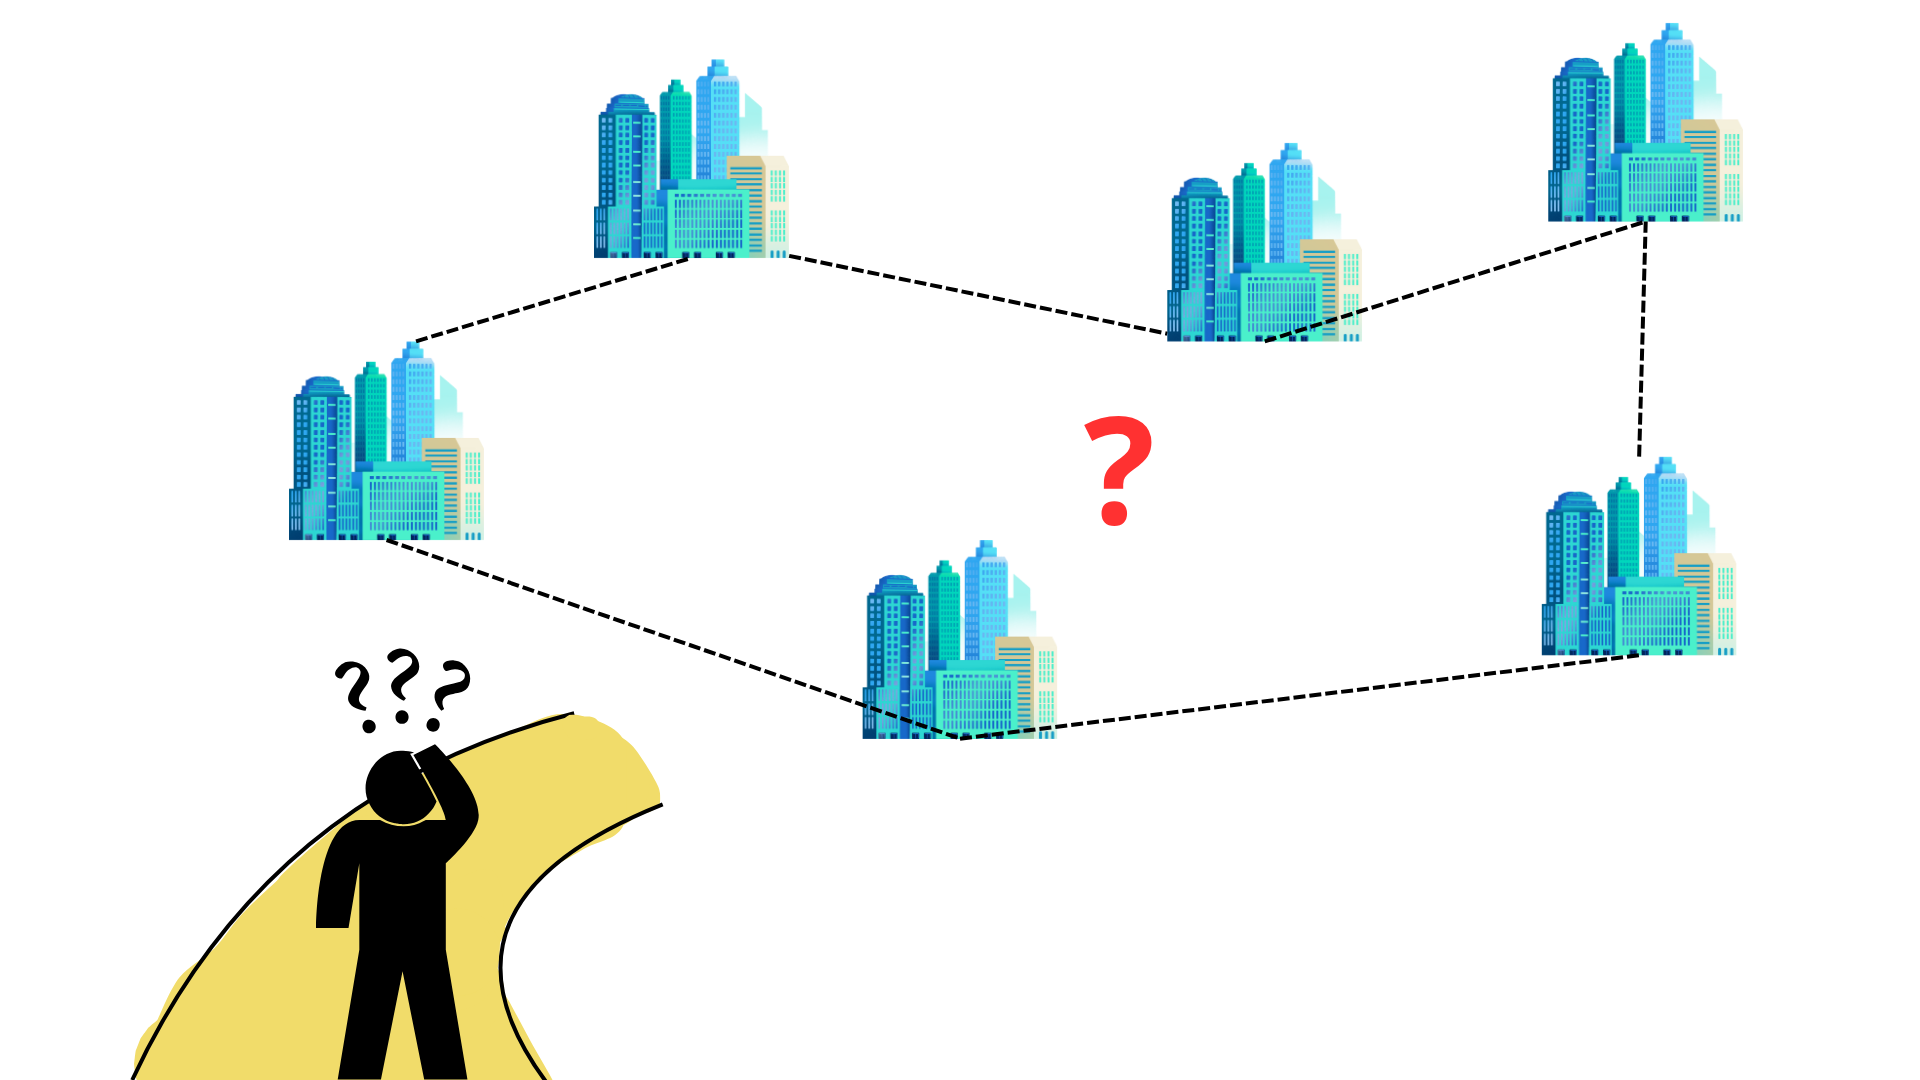
\includegraphics[width=0.65\textwidth]{rsc/img/intro/tsp.png}
    \caption{Planteamiento del problema del vendedor viajero (TSP).}\label{TSP}
\end{figure}

Este problema tiene múltiples aplicaciones prácticas en áreas como la logística, la planificación de rutas, la fabricación y la biología 
computacional, entre otras. Debido a su importancia teórica y práctica, ha motivado el desarrollo de diversos métodos de solución, desde 
algoritmos exactos basados en técnicas de ramificación y poda hasta heurísticas y metaheurísticas capaces de ofrecer buenas soluciones en 
tiempos razonables para instancias de gran tamaño.

Para esta ocasión, aplicaremos algoritmos genéticos para resolver este problema. Ya se ha explorado lo que son los algoritmos genéticos, 
su funcionamiento y sus aplicaciones en problemas de optimización por lo que lo abordaremos de manera más general en el contexto del TSP.\@

En este caso usaremos los métodos de cruce PMX y PBX, y las mutaciones de mezcla (scramble) y de intercambio de bloques (block transpose).

\subsection{Cruza PMX y PBX}
\subsubsection{PMX (Partially Mapped Crossover)}\label{intro_pmx}
El \textbf{PMX} o Cruce Parcialmente Mapeado es uno de los operadores de cruce más utilizados para el TSP.\@ Su principio fundamental es 
mantener el arreglo relativo de los genes de un padre mientras introduce variación del otro.

\subsubsection{Funcionamiento del PMX}

\begin{enumerate}
    \item \textbf{Selección de puntos de corte}: Se seleccionan aleatoriamente dos puntos de corte que dividen los cromosomas de los 
        padres en tres segmentos (izquierdo, medio y derecho).
    
    \item \textbf{Copia del segmento medio}: El segmento medio del primer padre se copia directamente al descendiente, preservando su 
        orden exacto.
    
    \item \textbf{Establecimiento de relaciones de mapeo}: Se crea una relación de mapeo entre los elementos del segmento medio de ambos
         padres para resolver conflictos.
    
    \item \textbf{Legalización del descendiente}: Se utiliza el mapeo para completar las posiciones restantes, asegurando que no haya 
        duplicaciones y que sea una permutación válida.
\end{enumerate}

\subsubsection{Ejemplo de PMX}

Consideremos los siguientes padres:
\begin{align}
\text{Padre 1} &= [1, 2, 3, 4, 5, 6, 7, 8, 9] \\
\text{Padre 2} &= [5, 4, 6, 9, 2, 1, 7, 8, 3]
\end{align}

Con puntos de corte en las posiciones 2 y 6, el segmento medio del Padre 1 es \([3, 4, 5, 6]\). Este segmento se copia al descendiente y se establece un mapeo con el segmento correspondiente del Padre 2 para completar las posiciones restantes sin duplicaciones.

\subsubsection{PBX (Position-Based Crossover)}

El \textbf{PBX} o Cruce Basado en Posición selecciona un subconjunto de posiciones del primer padre y preserva el orden relativo de los elementos restantes del segundo padre.

\subsubsection{Funcionamiento del PBX}\label{intro_pbx}

\begin{enumerate}
    \item \textbf{Selección aleatoria de posiciones}: Se seleccionan aleatoriamente varias posiciones (no necesariamente consecutivas) del primer padre.
    
    \item \textbf{Copia de elementos seleccionados}: Los elementos que se encuentran en las posiciones seleccionadas se copian directamente al descendiente en las mismas posiciones.
    
    \item \textbf{Eliminación de duplicados}: Se eliminan del segundo padre todos los elementos que ya fueron copiados.
    
    \item \textbf{Completado del descendiente}: Las posiciones restantes se llenan con los elementos sobrantes del segundo padre, manteniendo su orden relativo original.
\end{enumerate}

\subsubsection{Ejemplo de PBX}

Utilizando los mismos padres:
\begin{align}
\text{Padre 1} &= [1, 2, 3, 4, 5, 6, 7, 8, 9] \\
\text{Padre 2} &= [5, 4, 6, 9, 2, 1, 7, 8, 3]
\end{align}

Si se seleccionan las posiciones 3, 5 y 6 (correspondientes a los elementos 3, 5 y 6 del Padre 1) estos elementos se preservan en sus posiciones originales. Las posiciones restantes se completan con los elementos del Padre 2 que no han sido utilizados, manteniendo su orden relativo.


\subsection{Métodos de Mutación en el TSP}

En los algoritmos genéticos, la mutación es un operador que introduce diversidad en la población al modificar las rutas de manera controlada.
En este caso se decidieron utilizar los siguientes métodos de mutación debido a su efectividad en problemas de permutación como el TSP.\@:

\subsubsection{Mutación por Barajado (Scramble Mutation)}
Este método consiste en seleccionar un segmento de la ruta y reordenar de manera aleatoria las ciudades dentro de este segmento. 
De esta forma, la estructura global de la ruta se mantiene, pero el orden local de algunas ciudades cambia, lo que puede llevar 
a descubrir nuevas combinaciones con mejor aptitud. 

\textbf{Ejemplo:}
\[
[1,2,3,4,5,6,7,8] \quad \xrightarrow{\text{Scramble en } [3,4,5,6]} \quad [1,2,5,3,6,4,7,8]
\]

\subsubsection{Mutación por Transposición de Bloques (Block Transpose Mutation)}
En este método se eligen dos bloques de la ruta y se intercambian de lugar de manera directa. 
Esto modifica la posición relativa de grupos completos de ciudades, lo que nos permite explorar nuevas configuraciones manteniendo intacto 
el orden dentro de cada bloque.

\textbf{Ejemplo:}
\[
[1,2,3,4,5,6,7,8] \quad \xrightarrow{\text{Intercambiar } [2,3] \text{ con } [6,7]} \quad [1,6,7,4,5,2,3,8]
\]

\bigskip
Dicho de manera más sencilla \textit{scramble} altera el orden interno de un subconjunto de ciudades,
mientras que \textit{block transpose} cambia la posición relativa de segmentos completos de la ruta.

\subsection{Ciudades}\label{lista_ciudades}
Para este ejercicio se utilizaron las siguientes ciudades con su etiqueta correspondiente:
\begin{multicols}{3}
    \begin{itemize}
        \item 0 --- Mexico City
        \item 1 --- Quito
        \item 2 --- Miami
        \item 3 --- San Salvador
        \item 4 --- Mendoza
        \item 5 --- Guadalajara
        \item 6 --- Merida       
        \item 7 --- Washington D.C.
        \item 8 --- Monterrey
        \item 9 --- Managua     
        \item 10 --- Caracas
        \item 11 --- Boston      
        \item 12 --- Buenos Aires
        \item 13 --- New York
        \item 14 --- Panama City
        \item 15 --- Brasilia
        \item 16 --- Montevideo
        \item 17 --- Bogota
    \end{itemize}
\end{multicols}

\begin{figure}[H]
    \centering
    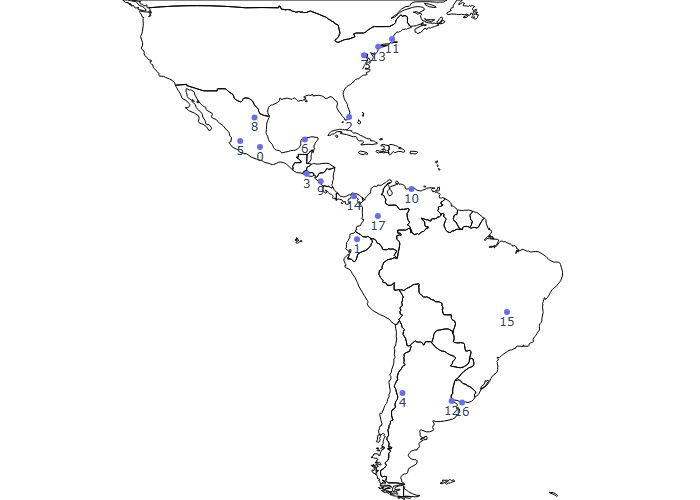
\includegraphics[width=0.85\textwidth]{rsc/img/intro/ciudades.png}
    \caption{Ciudades consideradas en el problema del vendedor viajero con su etiqueta.}\label{ciudades}
\end{figure}

\subsection{Cálculo de Distancias (Haversine)}\label{calculo_distancias}

Es importante mencionar que las coordenadas tomadas para este ejercicio fueron coordenadas geodesicas (latitud y longitud) y no coordenadas planas,
debido a que el uso de coordenadas planas puede introducir errores significativos en la estimación de distancias reales entre ciudades, dicho de 
otra manera podriamos estar tomando atajos que no existen en la realidad (Cortando la tierra por decirlo de una manera). 
Debido a esto la distancia entre dos ciudades se calculó usando la fórmula del haversine. Esta fórmula considera la curvatura de la Tierra y proporciona
una estimación más precisa de la distancia entre dos puntos geográficos. La fórmula del haversine es la siguiente:
\[
a = \sin^2\left(\frac{\Delta \phi}{2}\right) + \cos(\phi_1) \cdot \cos(\phi_2) \cdot \sin^2\left(\frac{\Delta \lambda}{2}\right)
\]

Con esto creamos una matriz de distancias entre todas las ciudades, que luego se utiliza para evaluar la aptitud de cada ruta en el algoritmo genético.